\documentclass[hyperref={pdfpagemode=FullScreen, colorlinks=false}]{beamer}

\usepackage{selinput}			% Inputencoding
	\SelectInputMappings{adieresis={ä}, germandbls={ß}, Euro={€}}
\usepackage[T1]{fontenc}		% Fontencoding
%
\usepackage{pifont}
\usepackage{csquotes,siunitx}			% Anführungszeichen; wird von biblatex gewünscht
\usepackage[backend=biber,citestyle=alphabetic,uniquelist=false]{biblatex}	% Literatur formatieren
\addbibresource{bodendynamik.bib}	% Literaturdatenbank
\usepackage{caption} 
\usepackage{subfig}
\usepackage{comment}
%%%%%%%%%%%%%%%%%%%%%%%%%%%%%%%%%%%%%%%%%%%%%%%%%%%%%%%%%%%%%%%%%%%%%%%%%%%%%%%%%%%%%%%%%%%%%%%%%%%%%%%
% Thema für Präsentation
\usetheme[fusszeile=ernstcolor,sprache=ngerman,seite=letzte,
verhaeltnis=16:10,
hausschrift=false,
navigation=false,
titelseite=blau]{TUBAF}

\TUBAFZweitlogo{
\includegraphics{fig_pdf/UFZ_logo_inv.pdf}}

%%%%%%%%%%%%%%%%%%%%%%%%%%%%%%%%%%%%%%%%%%%%%%%%%%%%%%%%%%%%%%%%%%%%%%%%%%%%%%%%%%%%%%%%%%%%%%%%%%%%%%%
% Optionen für Anmerkungen
\mode<presentation>{%
\setbeameroption{hide notes}				% keine Notizen (default)
%\setbeameroption{show notes}				% Notizen und Frames gemischt
%\setbeameroption{show only notes}			% nur Notizen
%
%\usepackage{pgfpages}					% wird für nachfolgendes benötigt
%\setbeameroption{show notes on second screen=left}	% wie gesagt; left, right, bottom, top
}




%%% DK packages and settings
\usepackage{amsmath}
\usepackage{pgfpages}
\pgfpagesuselayout{resize to}[a4paper, landscape]   % border shrink=5mm
\usepackage{siunitx}  
%\sisetup{locale = DE} 
\usepackage{tikz}
\usepackage{pgfplots}
\usepackage{animate}

\usetikzlibrary{math}
%\usetikzlibrary{datavisualization.formats.functions}
%\usetikzlibrary{datavisualization}
\usetikzlibrary{intersections}
\usepgfplotslibrary{groupplots,dateplot}
\pgfplotsset{compat=1.16}

\tikzset{
%DKspring(length) length=2...10
DKspring/.pic={
\coordinate (half_up) at (0.5*0.125*#1-0.5*0.125*2, 0.5*0.125*10-0.5*0.125*#1); %at (0.5*(#1-0.2), 0.5*(1.0-#1));
\coordinate (full_up)   at ( 0.125*#1-    0.125*2,     0.125*10-    0.125*#1);
\coordinate (full_down) at ( 0.125*#1-    0.125*2,    -0.125*10+    0.125*#1);
\draw (0, 0) -- ++(1, 0) -- ++(half_up)
    -- ++(full_down) -- ++(full_up) 
    -- ++(full_down) -- ++(full_up)
    -- ++(full_down) -- ++(full_up)
    -- ++(full_down) -- ++(half_up)
    -- ++(1, 0);
    },   
%DKdashpot(length) length=02...10    
DKdashpot/.pic={
\coordinate (upper_end) at (#1-0.5, 0.5);
\coordinate (lower_end) at (#1-0.5,-0.5);
\coordinate (upper_pos) at (#1-1, 0.5);
\coordinate (lower_pos) at (#1-1,-0.5);
\coordinate (center_pos) at (#1-1, 0.0);
\coordinate (center_end) at (#1, 0.0);
\draw (0, 0) -- ++(1, 0);
\draw (upper_end) -- (1, 0.5) -- (1, -0.5) -- (lower_end);
\draw (center_pos) -- (center_end);
\draw (upper_pos) -- (lower_pos);
    },
DKbase/.pic={
\draw[thick] (0, 1.5) -- (0, -1.5);
\foreach \y in {-1.5,-1.0,...,1.0} \draw[thin] (0, \y) -- +(-0.5, 0.5);
},
 invisible/.style={opacity=0},
  visible on/.style={alt={#1{}{invisible}}},
  alt/.code args={<#1>#2#3}{%
    \alt<#1>{\pgfkeysalso{#2}}{\pgfkeysalso{#3}} % \pgfkeysalso doesn't change the path
  }
}
\newlength\figH     % to scale tikzplotlib figures
\newlength\figW     % to scale tikzplotlib figures


\setbeamercovered{transparent}
%-----------------Custom footnote---------------
\TUBAFFzstrikttext{D. Kern \TUBAFfztrenner T. Nagel --- Vorlesung Bodendynamik --- Sommersemester 2021 }
%-----------------------------------------------

\tikzset{
%DKspring(length) length=2...10
DKspring/.pic={
\coordinate (half_up) at (0.5*0.125*#1-0.5*0.125*2, 0.5*0.125*10-0.5*0.125*#1); %at (0.5*(#1-0.2), 0.5*(1.0-#1));
\coordinate (full_up)   at ( 0.125*#1-    0.125*2,     0.125*10-    0.125*#1);
\coordinate (full_down) at ( 0.125*#1-    0.125*2,    -0.125*10+    0.125*#1);
\draw (0, 0) -- ++(1, 0) -- ++(half_up)
    -- ++(full_down) -- ++(full_up) 
    -- ++(full_down) -- ++(full_up)
    -- ++(full_down) -- ++(full_up)
    -- ++(full_down) -- ++(half_up)
    -- ++(1, 0);
    },   
%DKdashpot(length) length=02...10    
DKdashpot/.pic={
\coordinate (upper_end) at (#1-0.5, 0.5);
\coordinate (lower_end) at (#1-0.5,-0.5);
\coordinate (upper_pos) at (#1-1, 0.5);
\coordinate (lower_pos) at (#1-1,-0.5);
\coordinate (center_pos) at (#1-1, 0.0);
\coordinate (center_end) at (#1, 0.0);
\draw (0, 0) -- ++(1, 0);
\draw (upper_end) -- (1, 0.5) -- (1, -0.5) -- (lower_end);
\draw (center_pos) -- (center_end);
\draw (upper_pos) -- (lower_pos);
    },
DKbase/.pic={
\draw[thick] (0, 1.5) -- (0, -1.5);
\foreach \y in {-1.5,-1.0,...,1.0} \draw[thin] (0, \y) -- +(-0.5, 0.5);
},
 invisible/.style={opacity=0},
  visible on/.style={alt={#1{}{invisible}}},
  alt/.code args={<#1>#2#3}{%
    \alt<#1>{\pgfkeysalso{#2}}{\pgfkeysalso{#3}} % \pgfkeysalso doesn't change the path
  }
}


%%%%%%%%%%%%%%%%%%%%%%%%%%%%%%%%%%%%%%%%%%%%%%%%%%%%%%%%%%%%%%%%%%%%%%%%%%%%%%%%%%%%%%%%%%%%%%%%%%%%%%%
% Daten für die Titelseite:
%
% WICHTIG:	german shortcuts funktionieren nicht!! -> ÄäÖöÜüß verwenden
%		\\ fnkt nur im PM, \newline in AM und PM
%
\TUBAFTitel{Bodendynamik}

\TUBAFUntertitel{Dominik Kern, Thomas Nagel}

\TUBAFAutor[D. Kern | T. Nagel]{Dominik Kern, Thomas Nagel}

\TUBAFDatum[SS21]{Sommersemester 2021}

\TUBAFOrt[IFGT/BOME]{Institut für Geotechnik/Lehrstuhl fuer Bodenmechanik und Grundbau}

\TUBAFTitelseiteerlaeuterung{Lehrstuhl Bodenmechanik \& Grundbau\\Institut für Geotechnik\\[0.5cm]Vorlesung Sommersemester 2021}
	
%\TUBAFTitelseitebilder{
\includegraphics{title_page_pic_.jpg}}
%%%%%%%%%%%%%%%%%%%%%%%%%%%%%%%%%%%%%%%%%%%%%%%%%%%%%%%%%%%%%%%%%%%%%%%%%%%%%%%%%%%%%%%%%%%%%%%%%%%%%%%
% pdf-Infos setzen
\hypersetup{%
	pdfauthor={Dominik Kern},			% wird eigentlich von oben übernommen
	pdftitle={Bodendynamik}	% wird eigentlich von oben übernommen
}
%%%%%%%%%%%%%%%%%%%%%%%%%%%%%%%%%%%%%%%%%%%%%%%%%%%%%%%%%%%%%%%%%%%%%%%%%%%%%%%%%%%%%%%%%%%%%%%%%%%%%%%


\begin{document}
\maketitle

%\section{Wellenausbreitung im Untergrund}
\section{Elastisches dreidimensionales Kontinuum}

\begin{frame}
\frametitle{Übersicht}
\begin{center}

\includegraphics[width=0.2\textwidth]{fig_img/youtube.png}   
\end{center}

\href{https://www.youtube.com/watch?v=Za_22xo7ZQQ}{\textsl{IRIS Earthquake Science: 3-component Seismogram --- Capturing the motion of an earthquake.}}

\end{frame}

\begin{frame}
\frametitle{Mechanische Grundlagen}
Bodenverhalten, im einfachsten Fall isotrop, linear elastisches
\begin{align*}
 \sigma = ev + es
\end{align*}
Impulsbilanz damit
\begin{align*}
 \rho \ddot{a} =sigma
\end{align*}


\end{frame}


\subsection{Raumwellen}
% Vrettos2017
% Schmidt2017

\begin{frame}
\frametitle{Video}
\begin{center}

\includegraphics[width=0.2\textwidth]{fig_img/youtube.png}   
\end{center}


\href{https://www.youtube.com/watch?v=gjRGIpP-Qfw}{\textsl{Keith Miller: Demonstrating P and S Seismic Waves}}

\end{frame}


\begin{frame}
\frametitle{Vorbetrachtung}
\only<1>{
Wir betrachten zunächst eine in $x$-Richtung laufende, ebene Welle
\begin{align*}
 u(x,y,z,t)&=\bar{u}(x-ct),\\
 v(x,y,z,t)&=\bar{v}(x-ct),\\
 w(x,y,z,t)&=\bar{w}(x-ct),\\
\end{align*}
damit vereinfacht sich die Impulsbilanz zu
\begin{align*}
 \rho c^2 \bar{u}'' &= (\lambda+2\mu)\bar{u}'',\\
 \rho c^2 \bar{v}'' &= \mu \bar{v}'',\\
 \rho c^2 \bar{w}'' &= \mu \bar{w}''.
\end{align*}
}

\only<2>{
Diese vereinfachte Impulsbilanz 
\begin{align*}
 \rho c^2 \bar{u}'' &= (\lambda+2\mu)\bar{u}'',\\
 \rho c^2 \bar{v}'' &= \mu \bar{v}'',\\
 \rho c^2 \bar{w}'' &= \mu \bar{w}'',
\end{align*}
lässt zwei Lösungen zu
\begin{itemize}
 \item Longitudinalwelle $\bar{u}\ne 0$, $\bar{v}=0$, $\bar{w}= 0$ mit $c^2=\frac{\lambda+2\mu}{\rho}$ (P-Welle);
  \item Transversalwelle $\bar{u}= 0$, $\bar{v}\ne 0$, $\bar{w}\ne 0$ mit $c^2=\frac{\mu}{\rho}$ (S-Welle).
\end{itemize}
Anmerkung: Schubmodul $\mu$ und Steifemodul $\lambda+2\mu$
}

\only<3>{
\begin{figure}
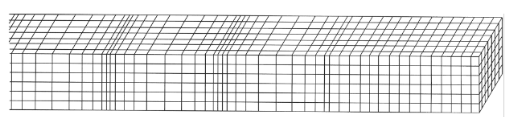
\includegraphics[width=0.9\textwidth]{fig_img/p_wave} 
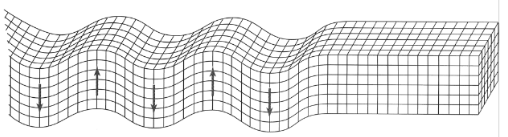
\includegraphics[width=0.9\textwidth]{fig_img/s_wave} 
\caption*{Kinematik ebener P-Welle (oben) und ebener S-Welle (unten) \cite{Vrettos2017}}
\end{figure}
}
\end{frame}


\begin{frame}
\frametitle{P-Wellen}
Erinnerung Impulsbilanz
\begin{align*}
 \rho \frac{\partial^2 u}{\partial t^2} &= (\lambda + \mu) \left( \frac{\partial^2 u}{\partial x^2} + \frac{\partial^2 v}{\partial y\, \partial x} + \frac{\partial^2 w}{\partial z\,\partial x} \right) + \mu \left( \frac{\partial^2 u}{\partial x^2} + \frac{\partial^2 u}{\partial y^2} + \frac{\partial^2 u}{\partial z^2} \right)
  &\quad& \bigg| \frac{\partial}{\partial x}
 \\
 \rho \frac{\partial^2 v}{\partial t^2} &= (\lambda + \mu) \left( \frac{\partial^2 u}{\partial x\,\partial y} + \frac{\partial^2 v}{\partial y^2} + \frac{\partial^2 w}{\partial z\,\partial x} \right)
 + \mu \left( \frac{\partial^2 v}{\partial x^2} + \frac{\partial^2 v}{\partial y^2} + \frac{\partial^2 v}{\partial z^2} \right)
 &\quad& \bigg| \frac{\partial}{\partial y}
 \\
 \rho \frac{\partial^2 w}{\partial t^2} &= (\lambda + \mu) \left( \frac{\partial^2 u}{\partial x\,\partial z} + \frac{\partial^2 v}{\partial y\, \partial z} + \frac{\partial^2 w}{\partial z^2} \right)
 + \mu \left( \frac{\partial^2 w}{\partial x^2} + \frac{\partial^2 w}{\partial y^2} + \frac{\partial^2 w}{\partial z^2} \right)
 &\quad& \bigg| \frac{\partial}{\partial z}
\end{align*}
\hrule \hfill {\small addieren}

\smallskip
\begin{equation*}
 \rho \frac{\partial^2 \varepsilon_V }{\partial t^2} = 
 (\lambda + 2 \mu) \left( \frac{\partial^2 \varepsilon_V }{\partial x^2} + \frac{\partial^2 \varepsilon_V }{\partial y^2}
 + \frac{\partial^2 \varepsilon_V }{\partial z^2} \right)
\end{equation*}

\end{frame}


\begin{frame}
\frametitle{S-Wellen}
Erinnerung Impulsbilanz ($x$-, $y$-Richtung)
\begin{align*}
 \rho \frac{\partial^2 u}{\partial t^2} &= (\lambda + \mu) \left( \frac{\partial^2 u}{\partial x^2} + \frac{\partial^2 v}{\partial y\, \partial x} + \frac{\partial^2 w}{\partial z\,\partial x} \right) + \mu \left( \frac{\partial^2 u}{\partial x^2} + \frac{\partial^2 u}{\partial y^2} + \frac{\partial^2 u}{\partial z^2} \right)
  &\quad& \bigg| \frac{\partial}{\partial y}
 \\
 \rho \frac{\partial^2 v}{\partial t^2} &= (\lambda + \mu) \left( \frac{\partial^2 u}{\partial x\,\partial y} + \frac{\partial^2 v}{\partial y^2} + \frac{\partial^2 w}{\partial z\,\partial x} \right)
 + \mu \left( \frac{\partial^2 v}{\partial x^2} + \frac{\partial^2 v}{\partial y^2} + \frac{\partial^2 v}{\partial z^2} \right)
 &\quad& \bigg| \frac{\partial}{\partial x}
\end{align*}
\hrule \hfill {\small subtrahieren}
\begin{equation*}
\rho \frac{\partial^2 \omega_z }{\partial t^2}
=\mu\left( \frac{\partial^2 \omega_z }{\partial x^2} + \frac{\partial^2 \omega_z }{\partial y^2}
 + \frac{\partial^2 \omega_z }{\partial z^2} \right)
\end{equation*}
mit \ $\omega_z=\frac{\partial v}{\partial x}-\frac{\partial u}{\partial y}$\,. Analog zwei weitere Gleichungen für $\omega_x$ und $\omega_y$.
\end{frame}


\begin{frame}
\frametitle{Reflexion am Rand}
\begin{columns}
\begin{column}[t]{.35\linewidth}
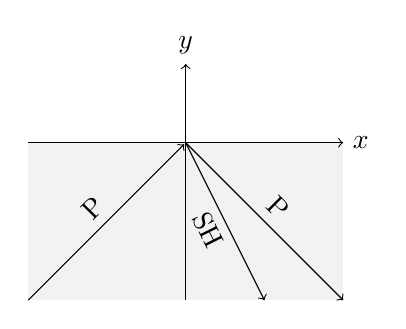
\begin{tikzpicture}
 \fill[black!5!white] (-2,0) rectangle (2,-2);
 \draw[->] (-2,0 ) -- (2,0) node[right] {$x$};
 \draw[->] ( 0,-2 ) -- (0,1) node[above] {$y$};
 \draw[->] (-2,-2) -- node[above, sloped] {P} (-0.02,-0.02);
 \draw[->] (0,0) -- node[below, sloped] {SH} (1, -2);
 \draw[->] (0,0) -- node[above, sloped] {P} (2, -2);
\end{tikzpicture}
         
\end{column}
\begin{column}[t]{.65\linewidth}
\vspace{-3.75cm}

\only<1>{
 Einfallende P-Welle
 \begin{equation*}
\mathbf{u}_1=\left[\begin{array}{c}
                    \sin\alpha_1 \\
                    \cos\alpha_1 \\
                    0
                   \end{array}\right]A_1
                   e^{i \kappa_1(x\sin\alpha_1+y\cos\alpha_1-c_P t)}
 \end{equation*}
 Reflektierte P- und SH-Welle
 \begin{align*}
 \mathbf{u}_2&=\left[\begin{array}{c}
                    \sin\alpha_2 \\
                    -\cos\alpha_2 \\
                    0
                   \end{array}\right]
                   A_2
                   e^{i \kappa_2(x\sin\alpha_2-y\cos\alpha_2-c_P t)}\\
\mathbf{u}_3&=\mathbf{e}_z\times\left[\begin{array}{c}
                    \sin\alpha_3 \\
                    -\cos\alpha_3 \\
                    0
                   \end{array}\right]
                   A_3
                   e^{i \kappa_3(x\sin\alpha_3-y\cos\alpha_3-c_S t)}
 \end{align*}
 }
\only<2>{
 Spannungsfreier Rand
 \begin{align*}
  \sigma_{xy}(x,0,z,t)&=0\\
  \sigma_{yy}(x,0,z,t)&=0
 \end{align*}
 Reflektierte P-Welle
 \begin{align*}
\alpha_1 &= \alpha_2\\
\kappa_1 &= \kappa_2
 \end{align*}
 Reflektierte SH-Welle
 \begin{equation*}
\frac{\sin\alpha_1}{\sin\alpha_3}=\frac{\kappa_3}{\kappa_1}=\frac{c_P}{c_S}
 \end{equation*}
 und Amplituden \dots \textsl{Details siehe Übung.}
 }
\end{column}
\end{columns}

\end{frame}


\begin{frame}
\frametitle{Reflexion/Transmission am Übergang}
\only<1>{
\begin{figure}
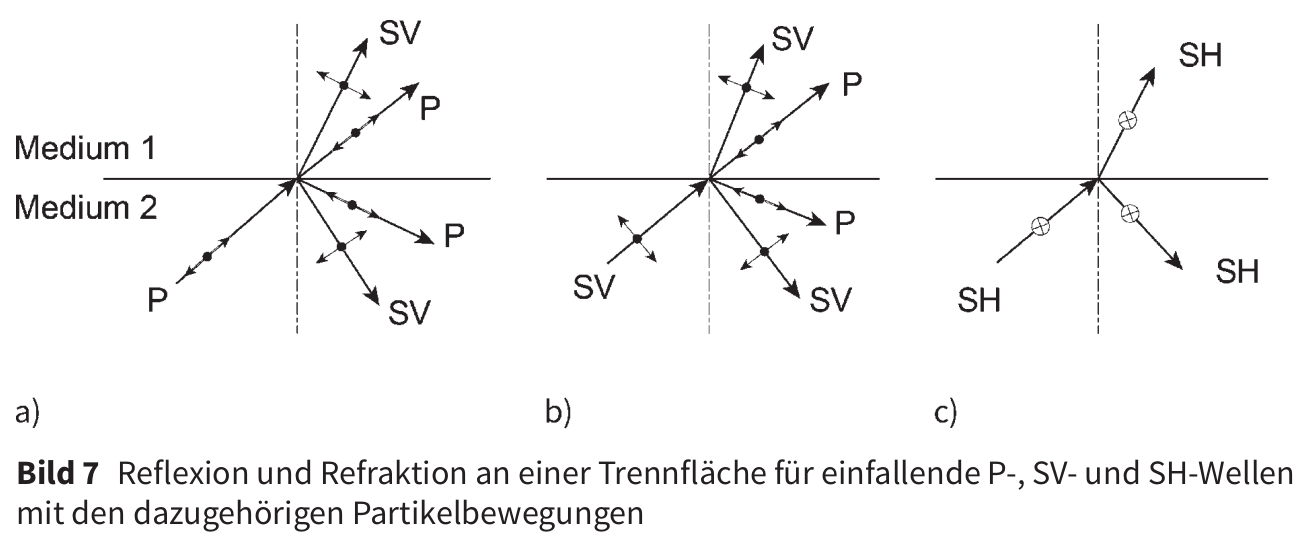
\includegraphics[width=1\textwidth]{fig_img/wave_transition} 
\caption*{Wellenausbreitung an einem diskontinuierlichen Übergang \cite{Vrettos2017}}
\end{figure}
}

\only<2>{
Die Richtungen der transmittierten und reflektierten Wellen lassen sich aus dem Snelliusschen Brechnungsgesetz 
$\dfrac{\sin\alpha}{c_\mathrm{ein}}
=\dfrac{\sin\beta}{c_\mathrm{ref}}
=\dfrac{\sin\gamma}{c_\mathrm{trans}}$ bestimmen.

\vfill
\begin{center}
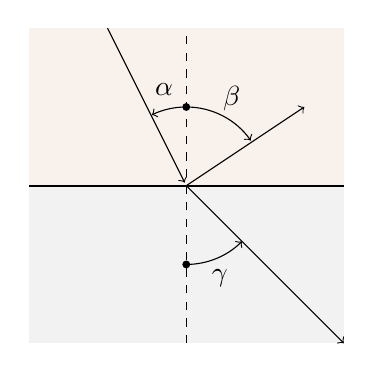
\begin{tikzpicture}
 \fill[brown!10!white] (-2,0) rectangle (2,2);
 \fill[black!5!white] (-2,0) rectangle (2,-2);
 \draw[thick] (-2,0 ) -- (2,0);
 \draw[->] (-1,2) -- (-0.02,0.04);
 \draw[->] (0,0) -- (1.5, 1);
 \draw[->] (0,0) -- (2, -2);
 \draw[dashed] (0,-2) -- (0,2);
 \draw[->] (0, 1) arc [start angle=90, end angle=116, radius=1];
 \draw (103:1.25) node {$\alpha$};
 \draw (62.5:1.25) node {$\beta$};
 \draw (290:1.25) node {$\gamma$};
 \draw[->] (0, 1) arc [start angle=90, end angle=35, radius=1];
 \draw[->] (0,-1) arc [start angle=270, end angle=315, radius=1];
 \fill (0, 1) circle [radius=0.05];
 \fill (0,-1) circle [radius=0.05];
\end{tikzpicture}
 
\end{center}
\vfill

Knobelspaß: Wie verteilen sich die Amplituden auf die transmittierten und reflektierten Anteile? Extraspaß: Was bedeuten Lösungen $\sin x >1$?
}

\end{frame}



\subsection{Oberflächenwellen}

\begin{frame}
\frametitle{Video}
\begin{center}

\includegraphics[width=0.2\textwidth]{fig_img/youtube.png}   
\end{center}

\href{https://www.youtube.com/watch?v=6yXgfYHAS7c}{\textsl{Wolfram: Propagation of Seismic Waves: Rayleigh waves}}

\href{https://www.youtube.com/watch?v=t7wJu0Kts7w}{\textsl{Wolfram: Propagation of Seismic Waves: Love waves}}

\end{frame}


\begin{frame}
\frametitle{Rayleigh Wellen}
Beschreibung, Dispersion,

\end{frame}


\begin{frame}
\frametitle{Kreisfundament}
Diskussion der Wellen

\end{frame}


\begin{frame}
\frametitle{Love Wellen}
Beschreibung
\end{frame}


\begin{frame}
\frametitle{Erdbeben}
siehe 1.5D
\end{frame}




\subsection{Abschließende Bemerkungen}
\begin{frame}
\frametitle{Zahlenwerte}
Fels, Sand
\end{frame}

\begin{frame}
\frametitle{Weitere Einflussfaktoren}
Tiefenabhängigkeit, Grundwasser/TPM,...
Inhomogenitäten
Beugung, Brechung
\end{frame}



%%%%%%%%%%%%%%%%%%%%%%%%%%%%%%%%%%%%%%%%%%%%%%%%

\section*{Literaturverzeichnis}

\begin{frame}[allowframebreaks]{}
	\printbibliography
\end{frame}
\end{document}
